\subsubsection{基于bigram的词包}
n-gram的模型特征可以作为文本的空间信息特征。
我们仍然使用scikit-learn的CountVectorizer模块来提取词包特征,不过这时的ngram\_range参数为(2, 2),表示我们使用bigram作为词包的基本单元。\\
我们抽出前几个bigram特征:['able get',
'able make',
'able see',
'able watch',
'absolute worst',
'absolutely brilliant',
'absolutely hilarious',
'absolutely love',
'absolutely loved',
'absolutely nothing'] \\
从这几个bigram特征可以预见到提取出的特征词包中有很多像副词那样的修饰词。\\
将提取到的bigram词包特征用来训练分类器模型,得到如下图\ref{fig:3crocbigram}所示的ROC曲线。
\begin{figure}[h]
\centering
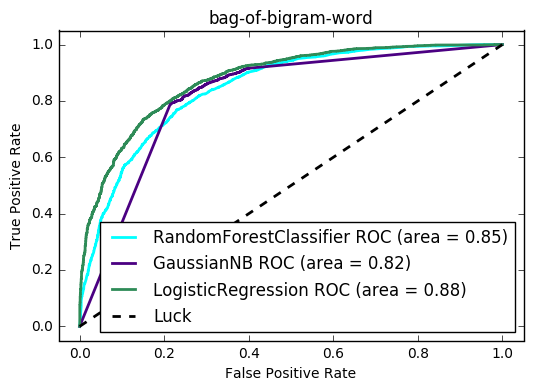
\includegraphics[width=0.9\linewidth]{3c_roc_bigram}
\caption[3c\_roc\_bigram]{三种模型用bigram词包的ROC曲线}
\label{fig:3crocbigram}
\end{figure}
从大体上我们可以看到,使用了bigram特征的分类器,其整体性能都比不使用bigram特征的分类器要差。
究其原因,我认为是像'absolutely'这样的副词修饰词占用了太多特征位置,导致其他一个词的强调词(或者那类一个词就可以鲜明地表达态度的词)没有成为词包中的频繁词,从而缺失了更有意义的单个词特征。\\